\documentclass[14pt,landscape]{report}

\usepackage[a4paper]{geometry}
\usepackage{amsmath}
\usepackage[myheadings]{fullpage}
\usepackage{fancyhdr}
%\usepackage{lastpage}
\usepackage{graphicx, wrapfig, subcaption, setspace, booktabs}

\pagestyle{empty} 
\begin{document}

\begin{figure}[p]
\centering
    \begin{subfigure}[t]{0.45\textwidth}
    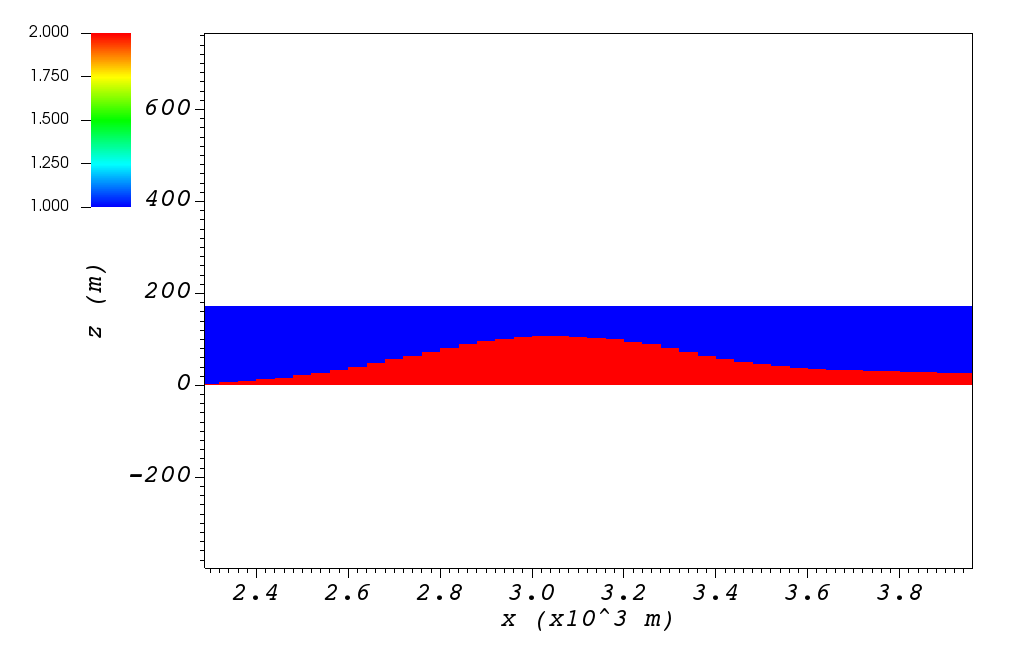
\includegraphics[width=\textwidth,keepaspectratio]{Images/askervein_y_3000_icell.png}
    \caption{}
    \end{subfigure}
	\begin{subfigure}[t]{0.45\textwidth}
    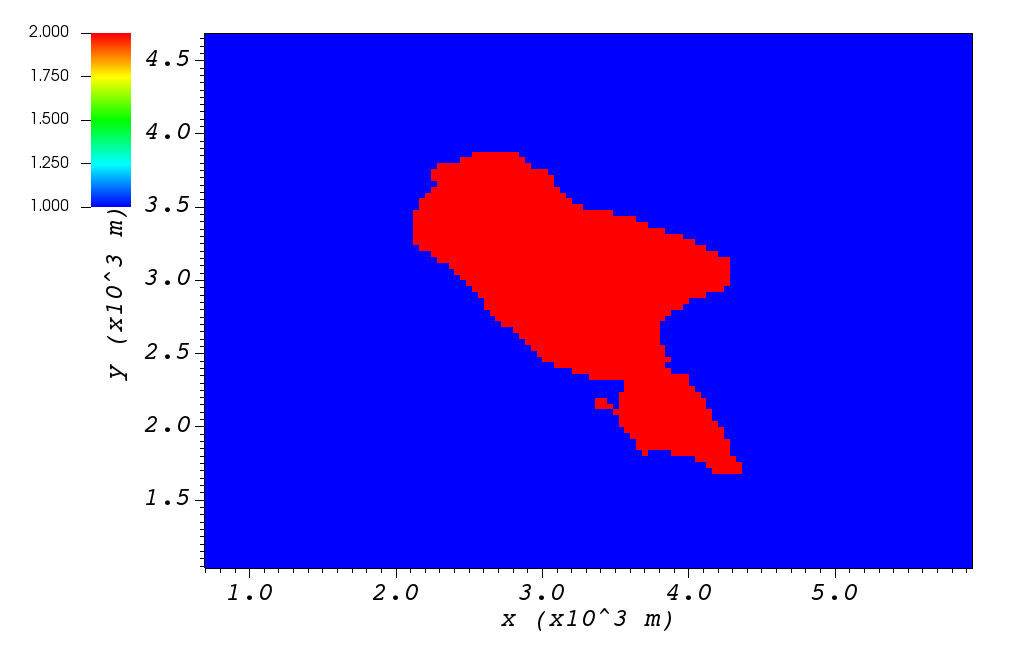
\includegraphics[width=\textwidth,keepaspectratio]{Images/askervein_z_20_icell.png}
    \caption{}
    \end{subfigure}
\end{figure}

\begin{figure}[p]
    \centering
    \begin{subfigure}[t]{0.45\textwidth}
    \centering
    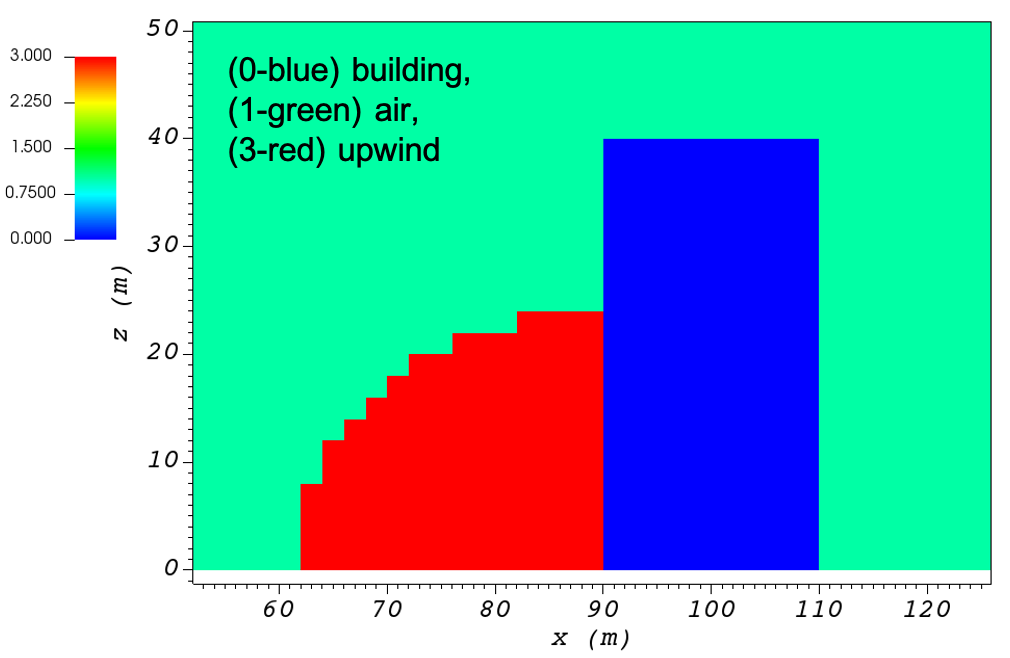
\includegraphics[width=10.3cm,keepaspectratio]{Images/upwind_y_100_1_init_icell.png}
    \caption{Cell type}
    \end{subfigure}
    \begin{subfigure}[t]{0.45\textwidth}
    \centering
    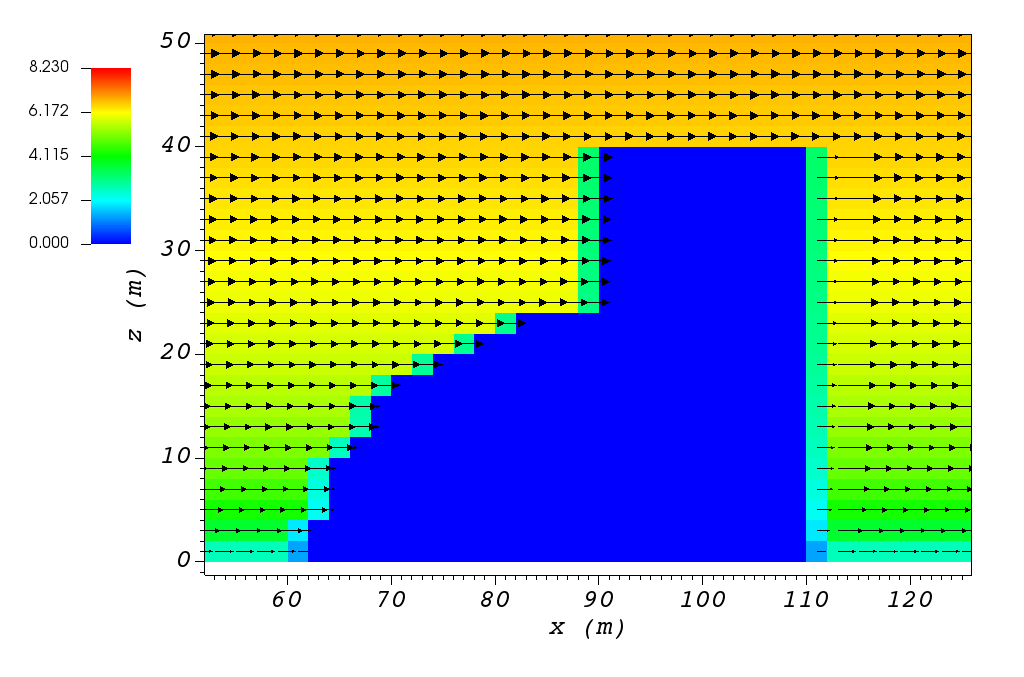
\includegraphics[width=11.0cm,keepaspectratio]{Images/upwind_y_100_1_init_vel.png}
    \caption{Initial velocity field}
    \end{subfigure}
    \begin{subfigure}[t]{0.45\textwidth}
    \centering
    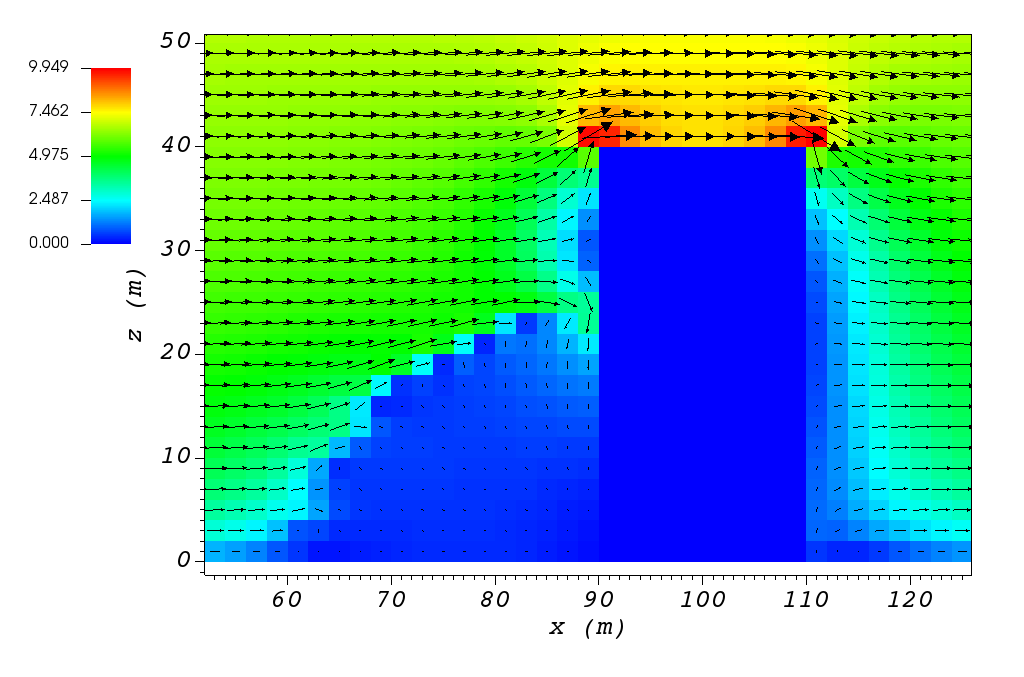
\includegraphics[width=11.0cm,keepaspectratio]{Images/upwind_y_100_1_final.png}
    \caption{Final velocity field}
    \end{subfigure}
\end{figure}
\begin{figure}[p]
    \centering
    \begin{subfigure}[t]{0.45\textwidth}
    \centering
    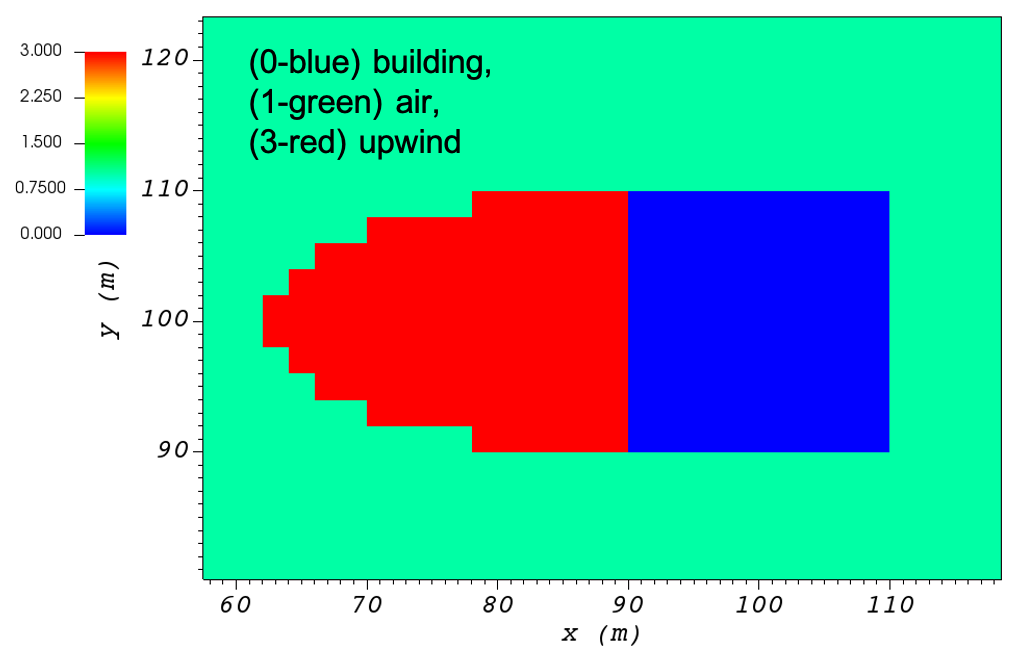
\includegraphics[width=10.3cm,keepaspectratio]{Images/upwind_z_5_1_init_icell.png}
    \caption{Cell type}
    \end{subfigure}
    \begin{subfigure}[t]{0.45\textwidth}
    \centering
    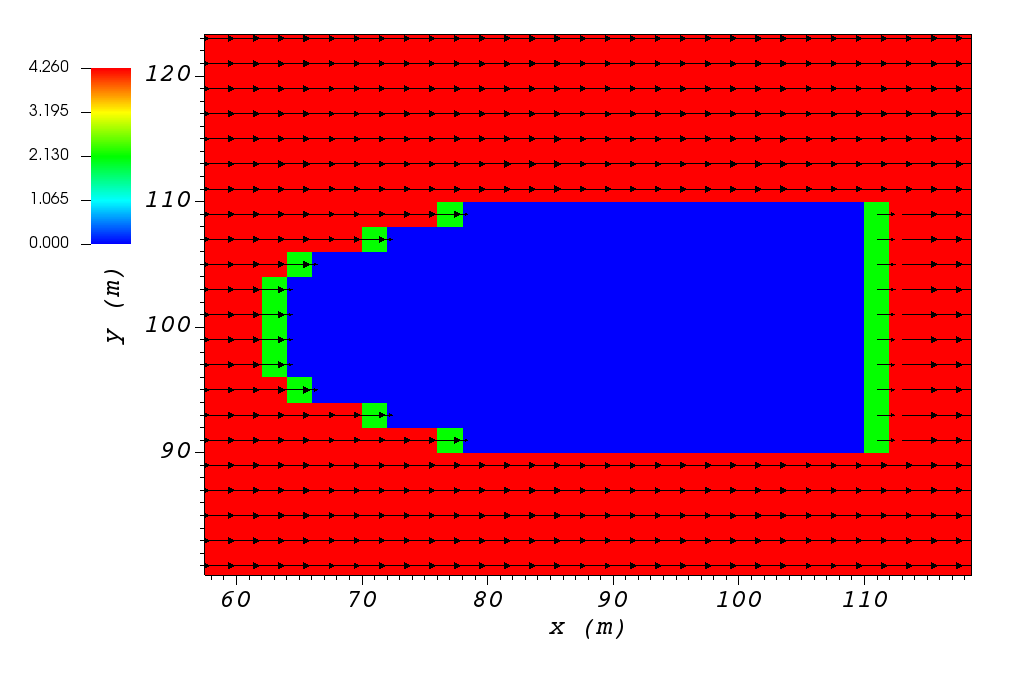
\includegraphics[width=11.0cm,keepaspectratio]{Images/upwind_z_5_1_init_vel.png}
    \caption{Initial velocity field}
    \end{subfigure}
    \begin{subfigure}[t]{0.45\textwidth}
    \centering
    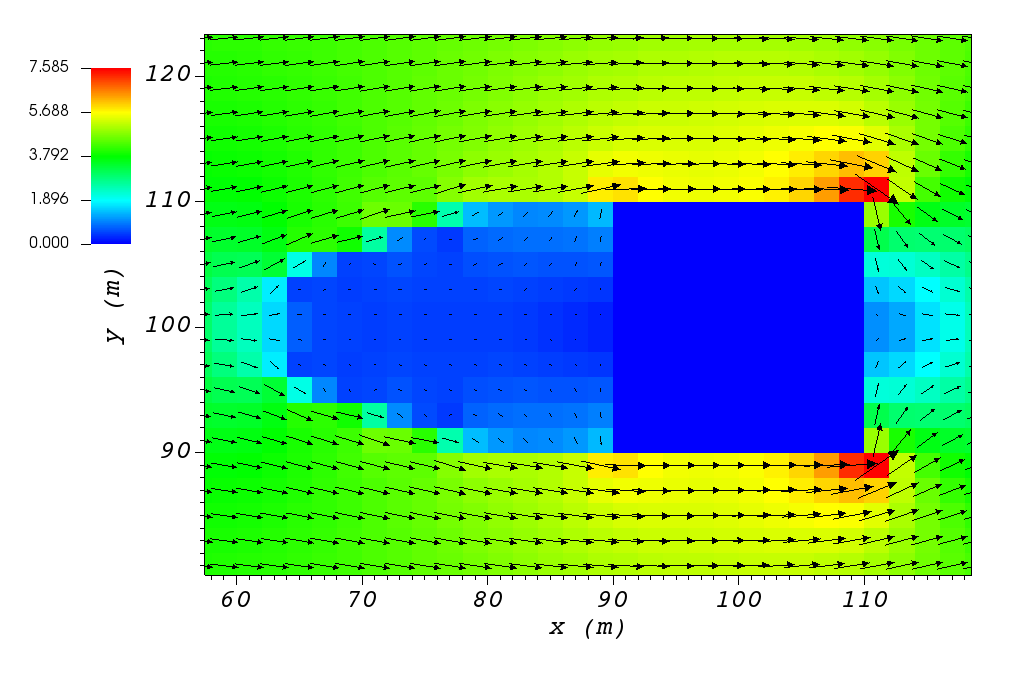
\includegraphics[width=11.0cm,keepaspectratio]{Images/upwind_z_5_1_final.png}
    \caption{Final velocity field}
    \end{subfigure}
\end{figure}



\begin{figure}[p]
    \centering
    \begin{subfigure}[t]{0.45\textwidth}
    \centering
    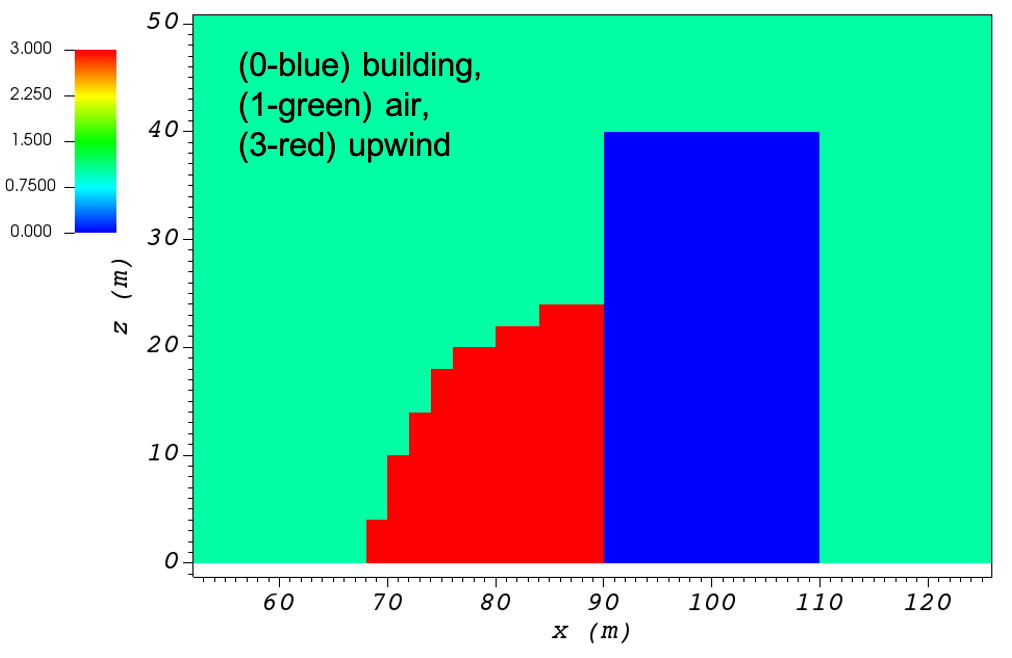
\includegraphics[width=10.3cm,keepaspectratio]{Images/upwind_y_100_2_init_icell.png}
    \caption{Cell type}
    \end{subfigure}
    \begin{subfigure}[t]{0.45\textwidth}
    \centering
    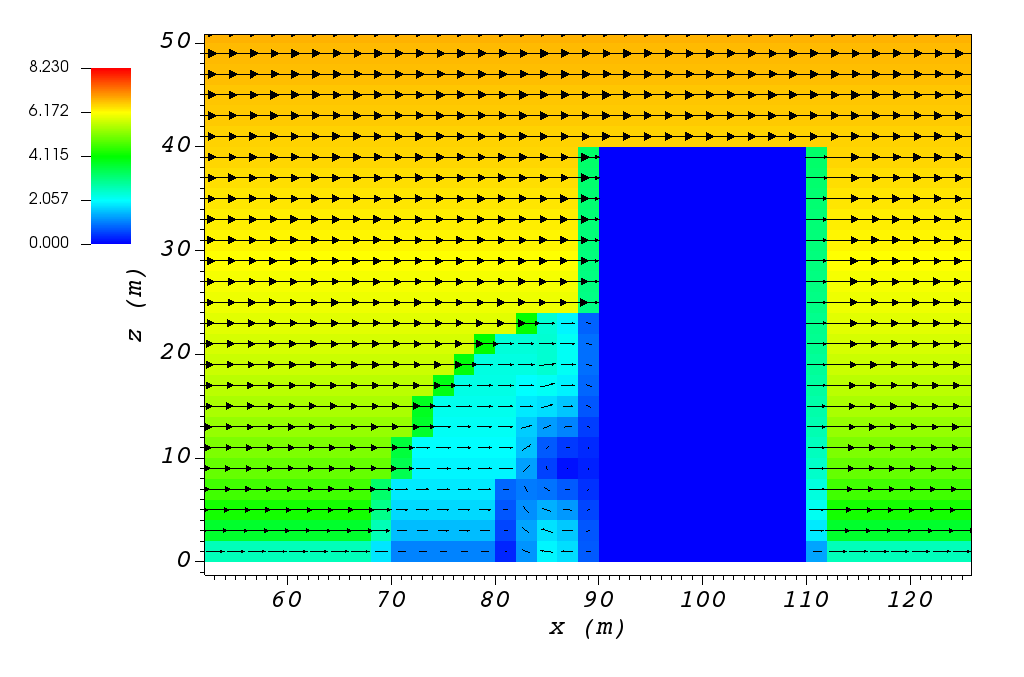
\includegraphics[width=11.0cm,keepaspectratio]{Images/upwind_y_100_2_init_vel.png}
    \caption{Initial velocity field}
    \end{subfigure}
    \begin{subfigure}[t]{0.45\textwidth}
    \centering
    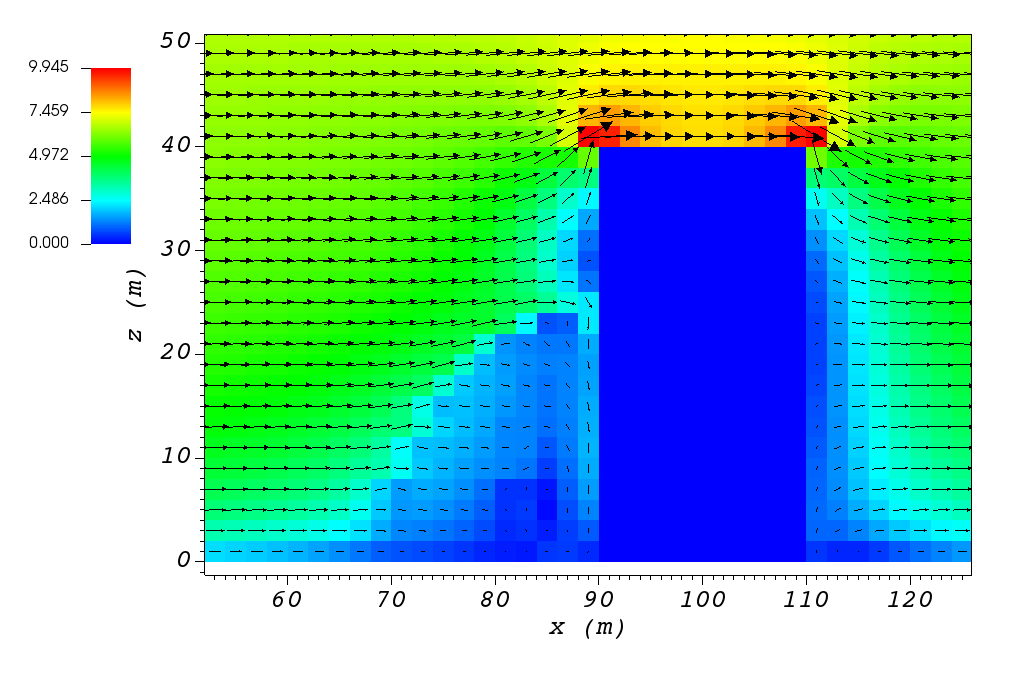
\includegraphics[width=11.0cm,keepaspectratio]{Images/upwind_y_100_2_final.png}
    \caption{Final velocity field}
    \end{subfigure}
\end{figure}
\begin{figure}[p]
    \centering
    \begin{subfigure}[t]{0.45\textwidth}
    \centering
    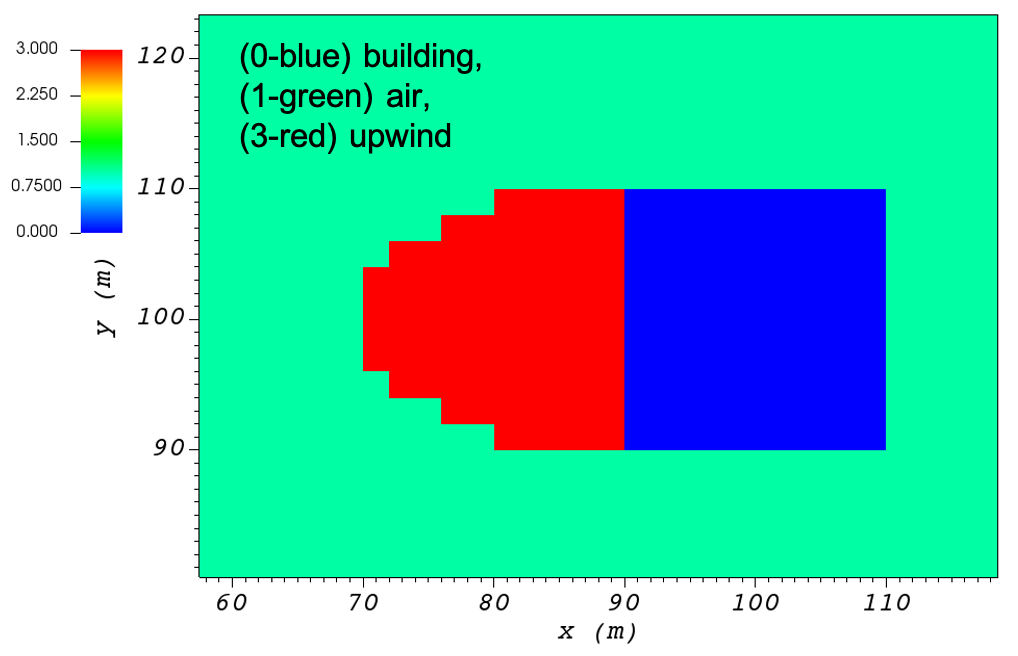
\includegraphics[width=10.3cm,keepaspectratio]{Images/upwind_z_5_2_init_icell.png}
    \caption{Cell type}
    \end{subfigure}
    \begin{subfigure}[t]{0.45\textwidth}
    \centering
    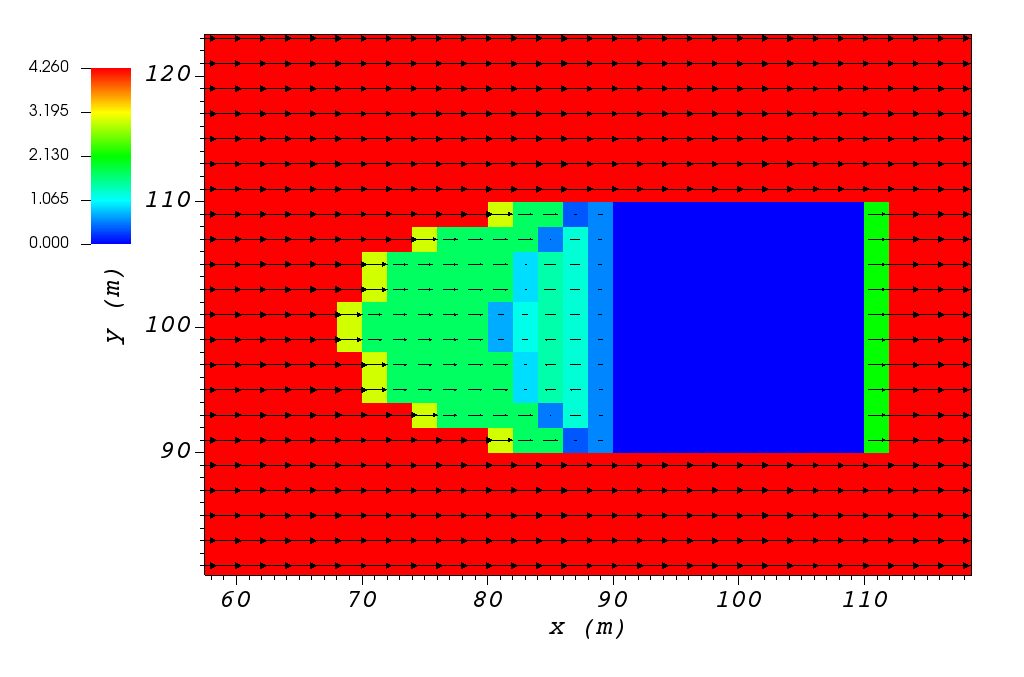
\includegraphics[width=11.0cm,keepaspectratio]{Images/upwind_z_5_2_init_vel.png}
    \caption{Initial velocity field}
    \end{subfigure}
    \begin{subfigure}[t]{0.45\textwidth}
    \centering
    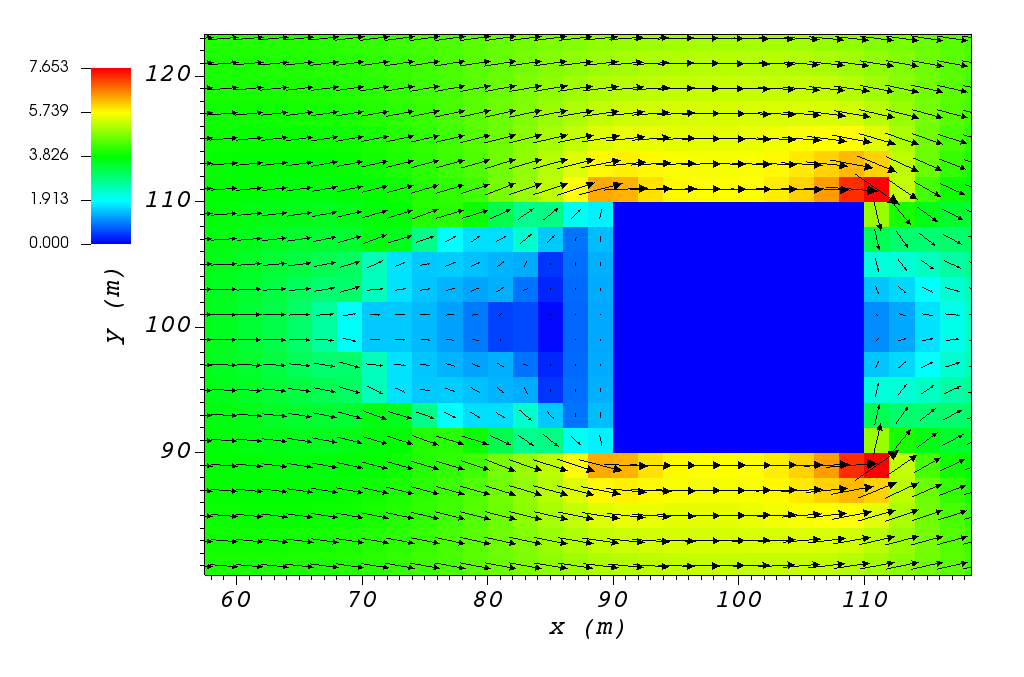
\includegraphics[width=11.0cm,keepaspectratio]{Images/upwind_z_5_2_final.png}
    \caption{Final velocity field}
    \end{subfigure}
\end{figure}



\begin{figure}[p]
    \centering
    \begin{subfigure}[t]{0.45\textwidth}
    \centering
    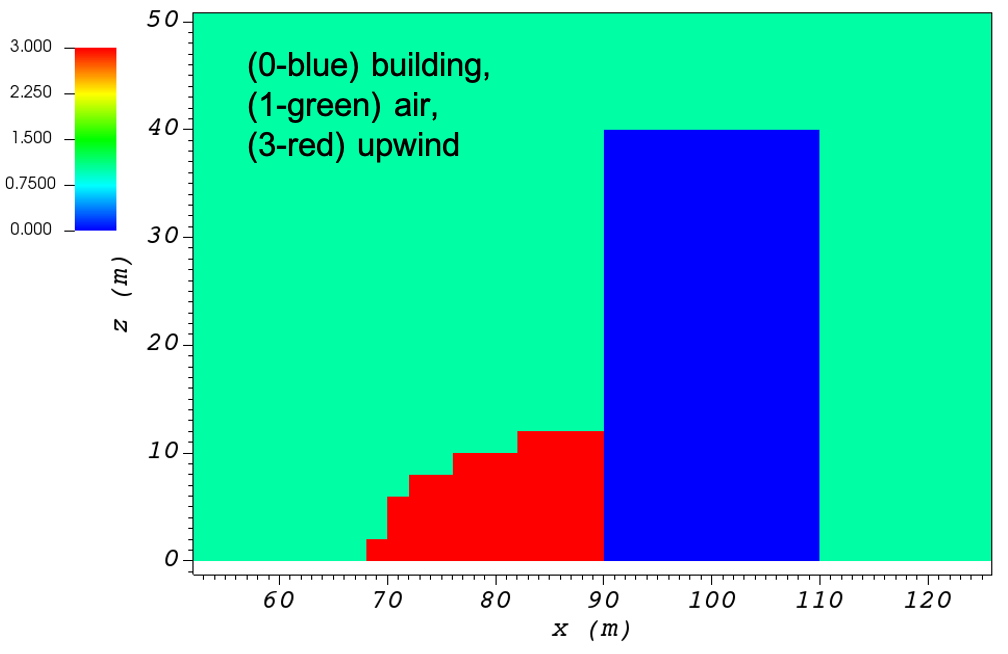
\includegraphics[width=10.3cm,keepaspectratio]{Images/upwind_y_100_3_init_icell.png}
    \caption{Cell type}
    \end{subfigure}
    \begin{subfigure}[t]{0.45\textwidth}
    \centering
    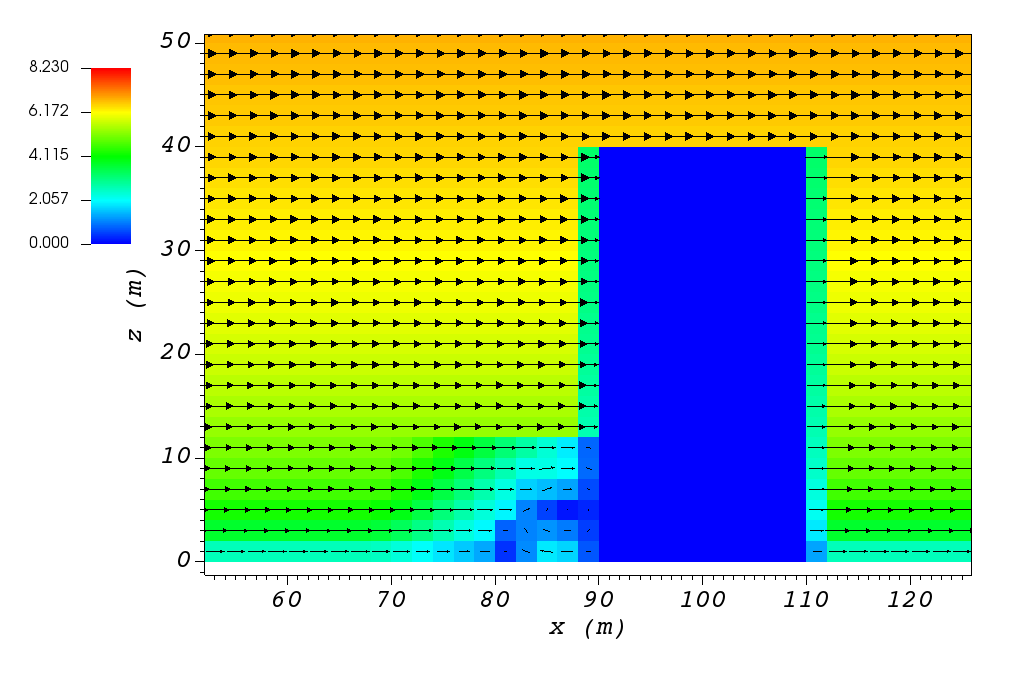
\includegraphics[width=11.0cm,keepaspectratio]{Images/upwind_y_100_3_init_vel.png}
    \caption{Initial velocity field}
    \end{subfigure}
    \begin{subfigure}[t]{0.45\textwidth}
    \centering
    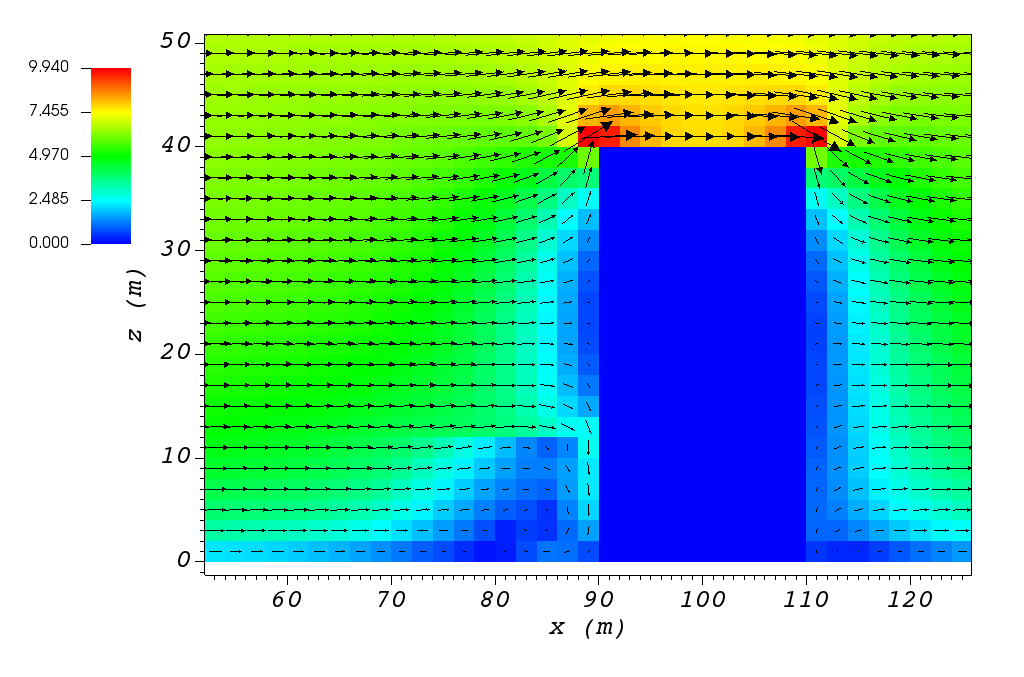
\includegraphics[width=11.0cm,keepaspectratio]{Images/upwind_y_100_3_final.png}
    \caption{Final velocity field}
    \end{subfigure}
\end{figure}
\begin{figure}[p]
    \centering
    \begin{subfigure}[t]{0.45\textwidth}
    \centering
    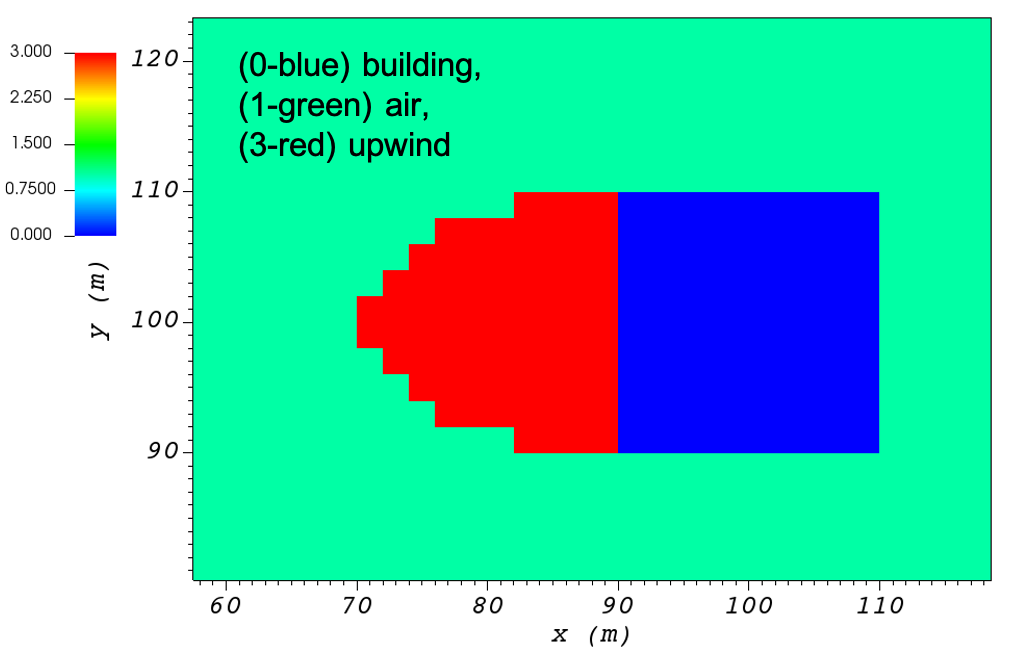
\includegraphics[width=10.3cm,keepaspectratio]{Images/upwind_z_5_3_init_icell.png}
    \caption{Cell type}
    \end{subfigure}
    \begin{subfigure}[t]{0.45\textwidth}
    \centering
    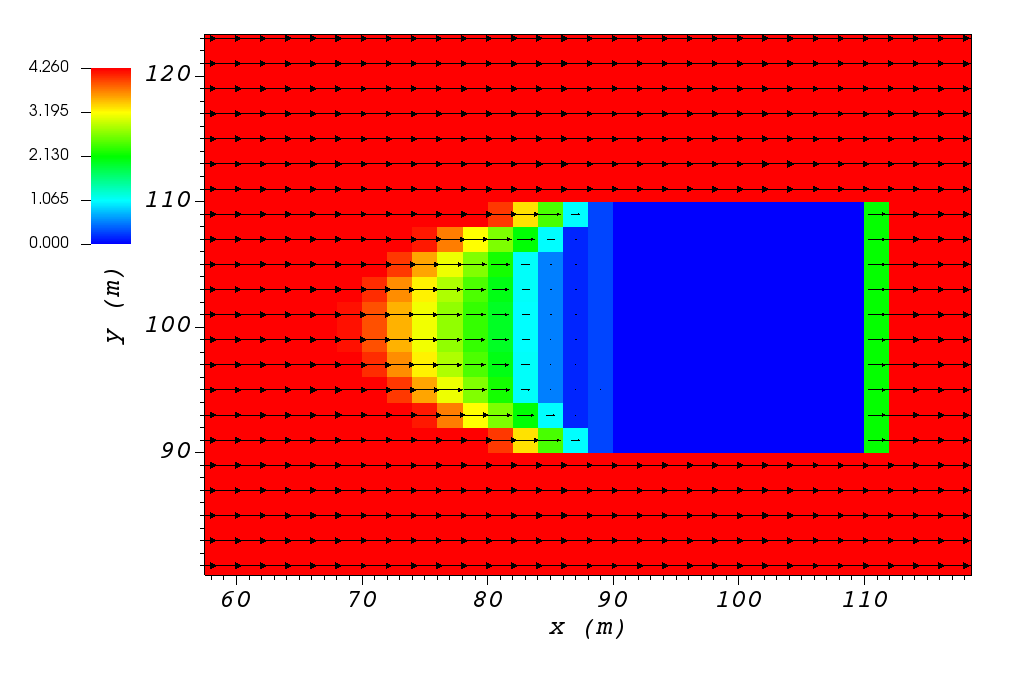
\includegraphics[width=11.0cm,keepaspectratio]{Images/upwind_z_5_3_init_vel.png}
    \caption{Initial velocity field}
    \end{subfigure}
    \begin{subfigure}[t]{0.45\textwidth}
    \centering
    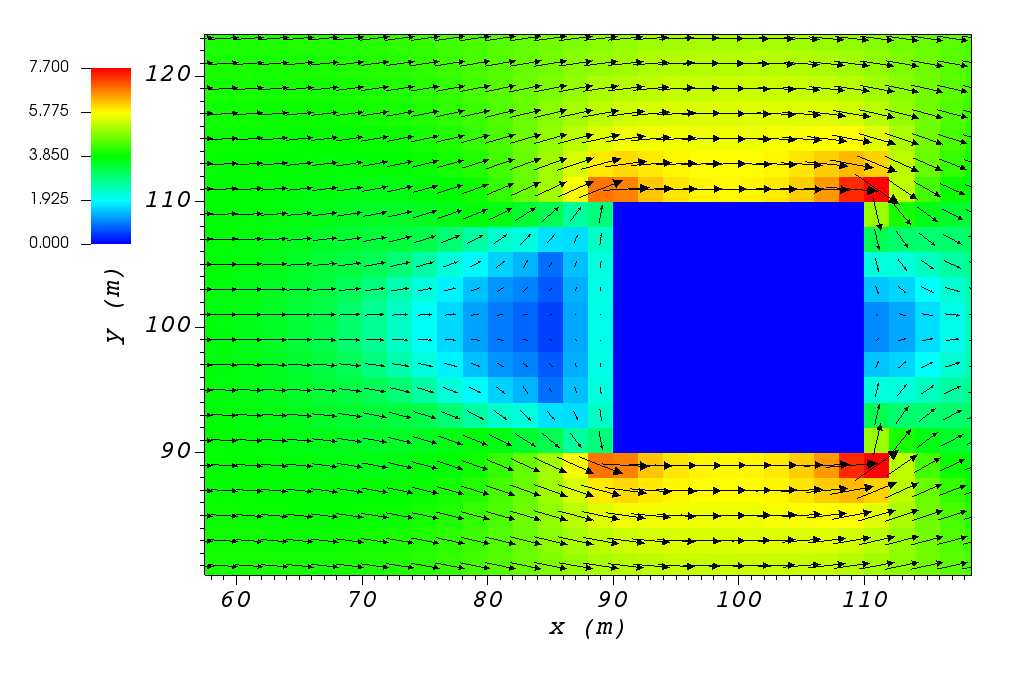
\includegraphics[width=11.0cm,keepaspectratio]{Images/upwind_z_5_3_final.png}
    \caption{Final velocity field}
    \end{subfigure}
\end{figure}


\begin{figure}[p]
    \centering
    \begin{subfigure}[t]{0.45\textwidth}
    \centering
    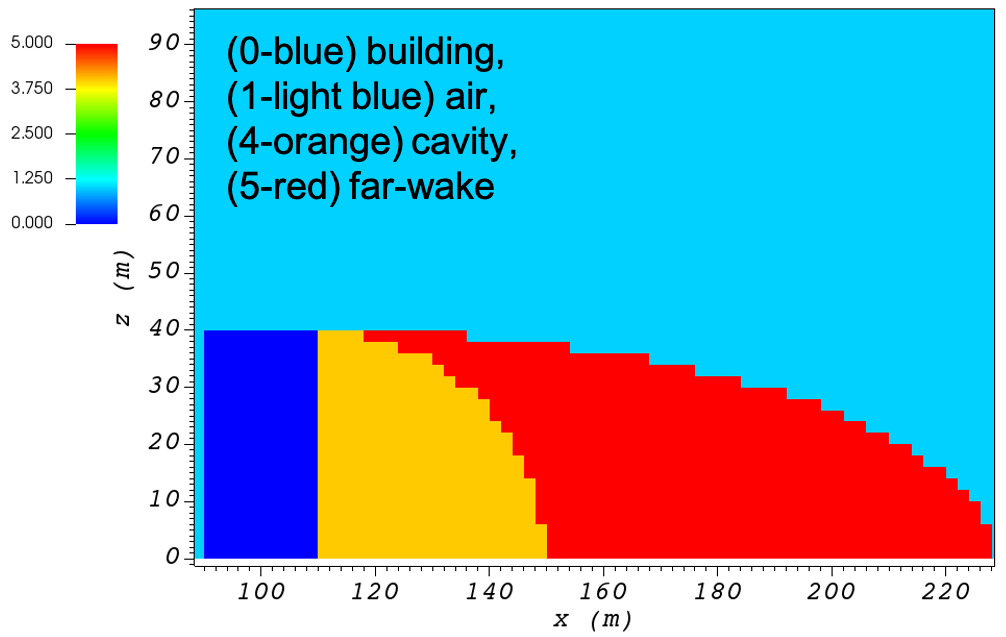
\includegraphics[width=10.3cm,keepaspectratio]{Images/wake_y_100_1_init_icell.png}
    \caption{Cell type}
    \end{subfigure}
    \begin{subfigure}[t]{0.45\textwidth}
    \centering
    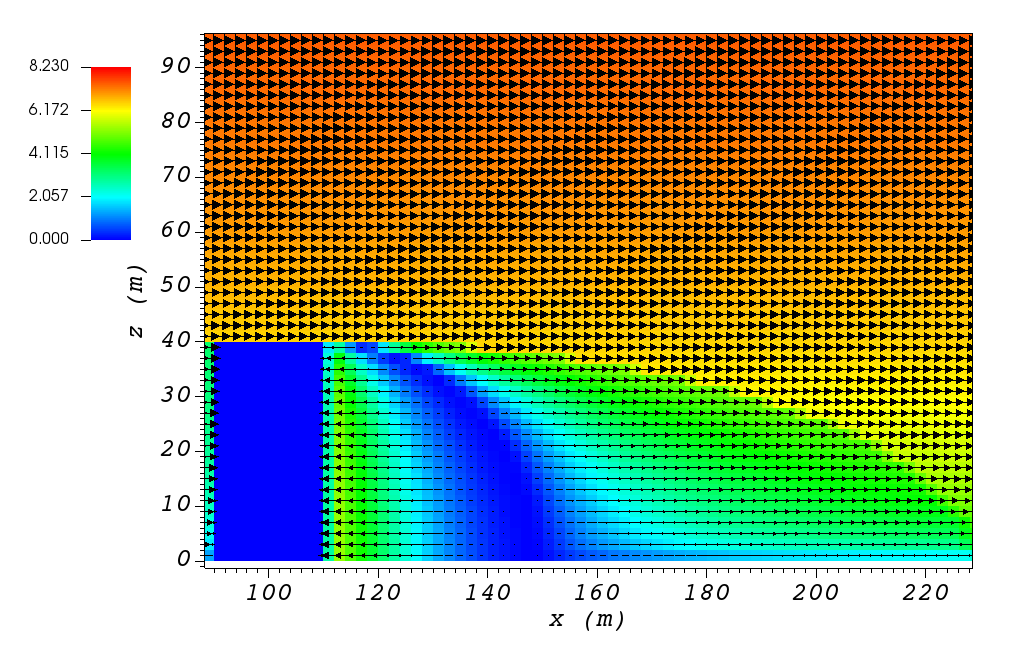
\includegraphics[width=11.0cm,keepaspectratio]{Images/wake_y_100_1_init_vel.png}
    \caption{Initial velocity field}
    \end{subfigure}
    \begin{subfigure}[t]{0.45\textwidth}
    \centering
    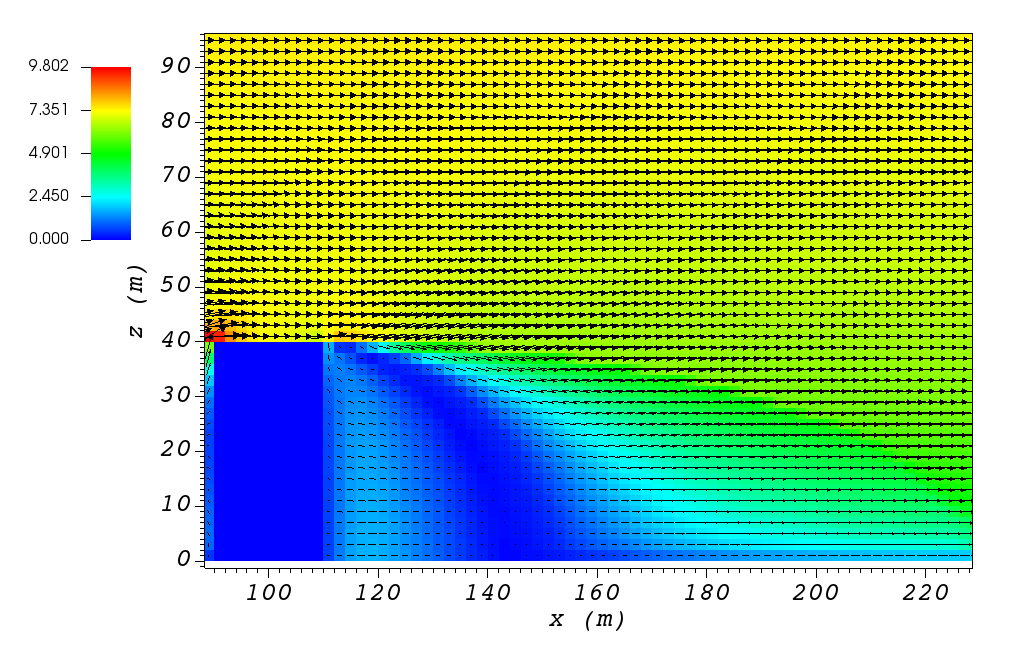
\includegraphics[width=11.0cm,keepaspectratio]{Images/wake_y_100_1_final.png}
    \caption{Final velocity field}
    \end{subfigure}
\end{figure}
\begin{figure}[p]
    \centering
    \begin{subfigure}[t]{0.45\textwidth}
    \centering
    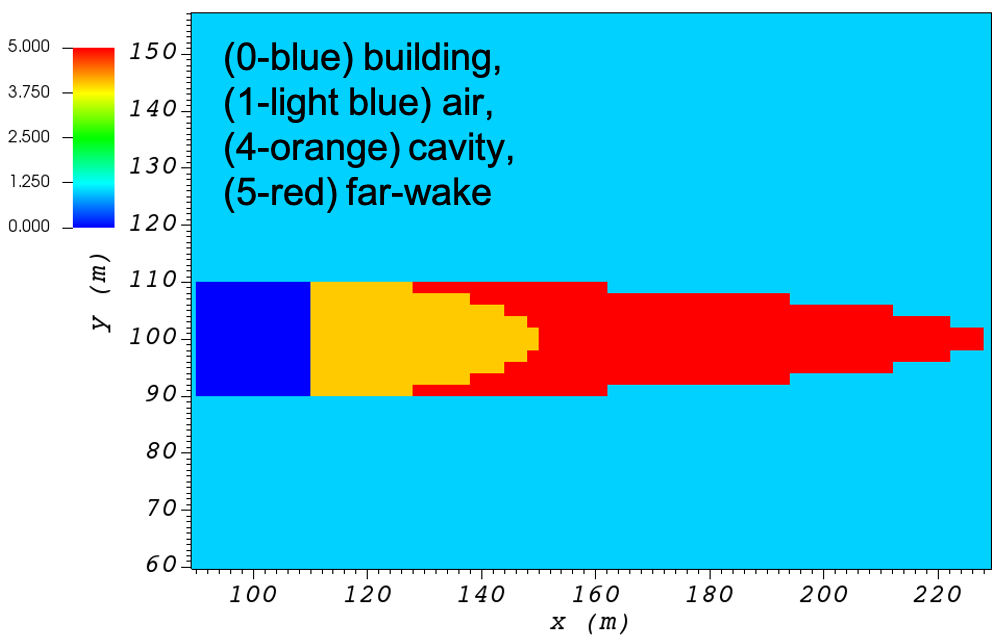
\includegraphics[width=10.3cm,keepaspectratio]{Images/wake_z_5_1_init_icell.png}
    \caption{Cell type}
    \end{subfigure}
    \begin{subfigure}[t]{0.45\textwidth}
    \centering
    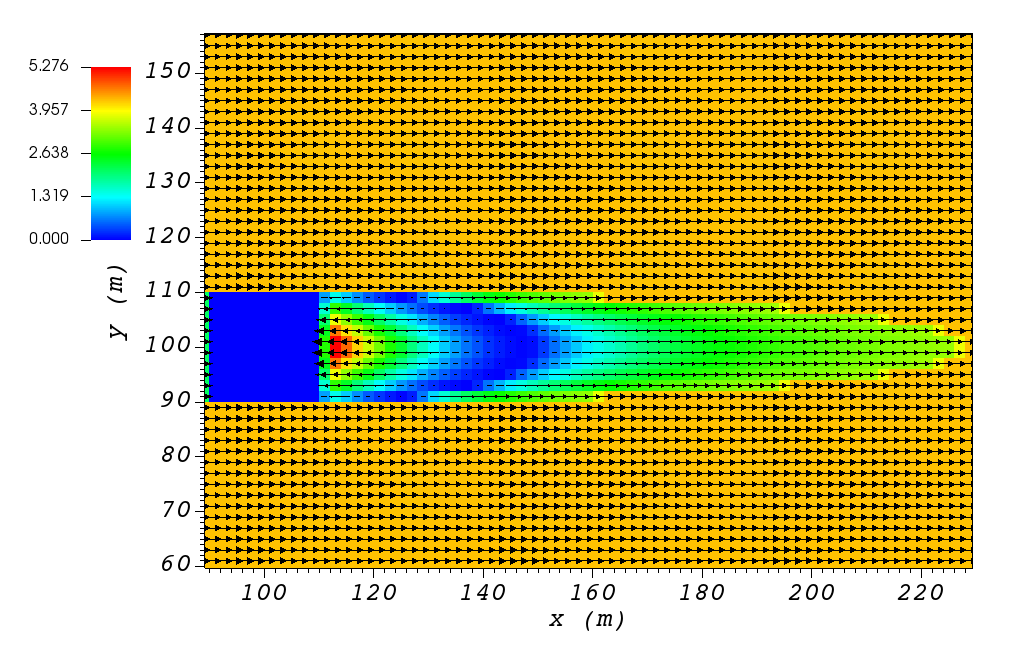
\includegraphics[width=11.0cm,keepaspectratio]{Images/wake_z_5_1_init_vel.png}
    \caption{Initial velocity field}
    \end{subfigure}
    \begin{subfigure}[t]{0.45\textwidth}
    \centering
    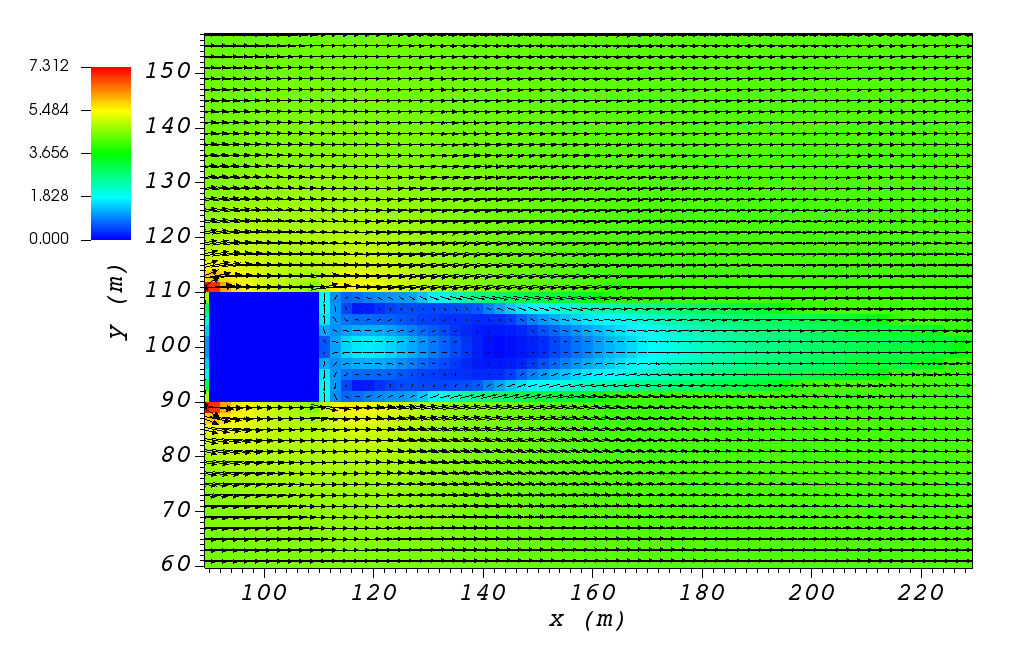
\includegraphics[width=11.0cm,keepaspectratio]{Images/wake_z_5_1_final.png}
    \caption{Final velocity field}
    \end{subfigure}
\end{figure}



\begin{figure}[p]
    \centering
    \begin{subfigure}[t]{0.45\textwidth}
    \centering
    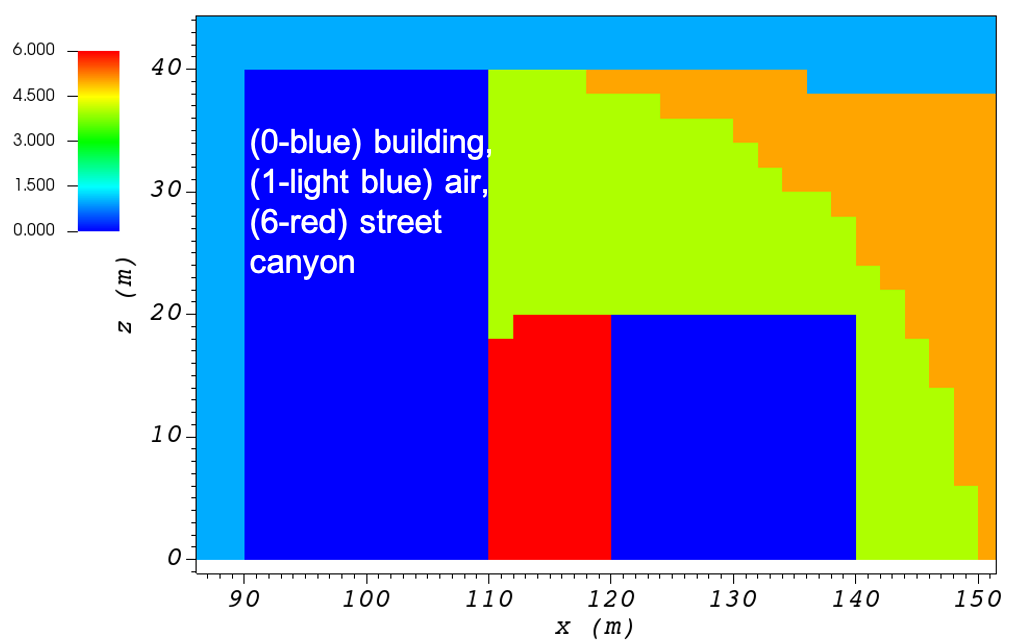
\includegraphics[width=10.3cm,keepaspectratio]{Images/street_y_100_1_init_icell.png}
    \caption{Cell type}
    \end{subfigure}
    \begin{subfigure}[t]{0.45\textwidth}
    \centering
    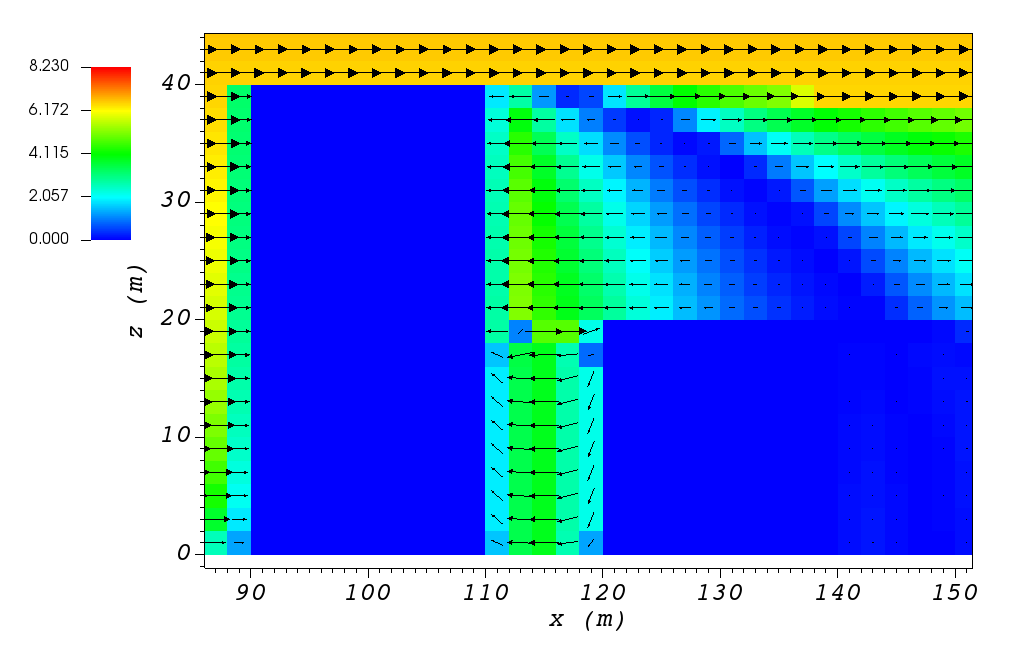
\includegraphics[width=11.0cm,keepaspectratio]{Images/street_y_100_1_init_vel.png}
    \caption{Initial velocity field}
    \end{subfigure}
    \begin{subfigure}[t]{0.45\textwidth}
    \centering
    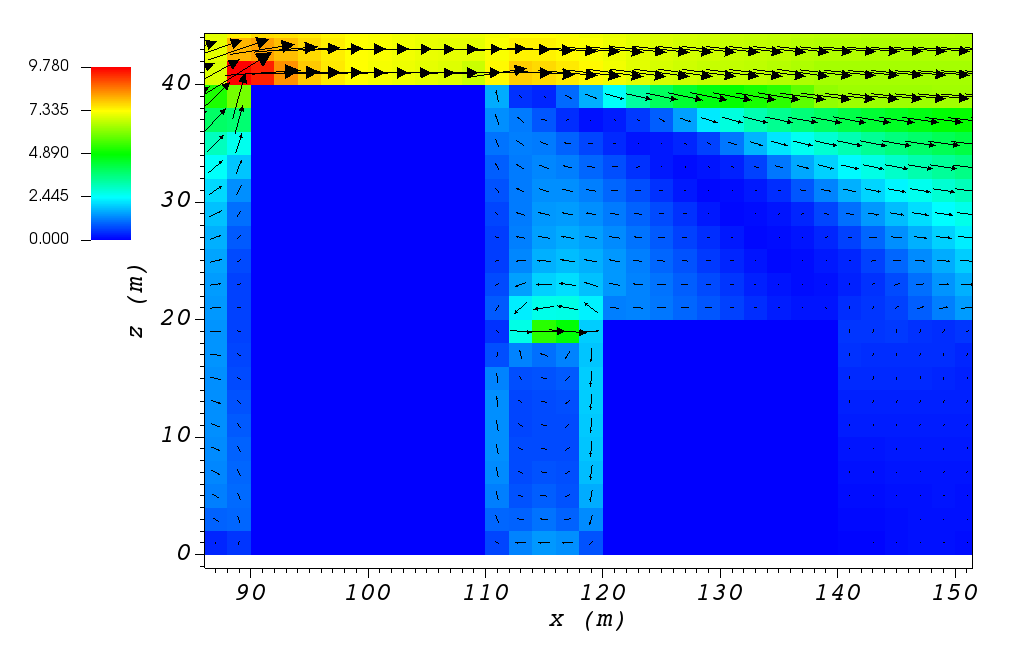
\includegraphics[width=11.0cm,keepaspectratio]{Images/street_y_100_1_final.png}
    \caption{Final velocity field}
    \end{subfigure}
\end{figure}
\begin{figure}[p]
    \centering
    \begin{subfigure}[t]{0.45\textwidth}
    \centering
    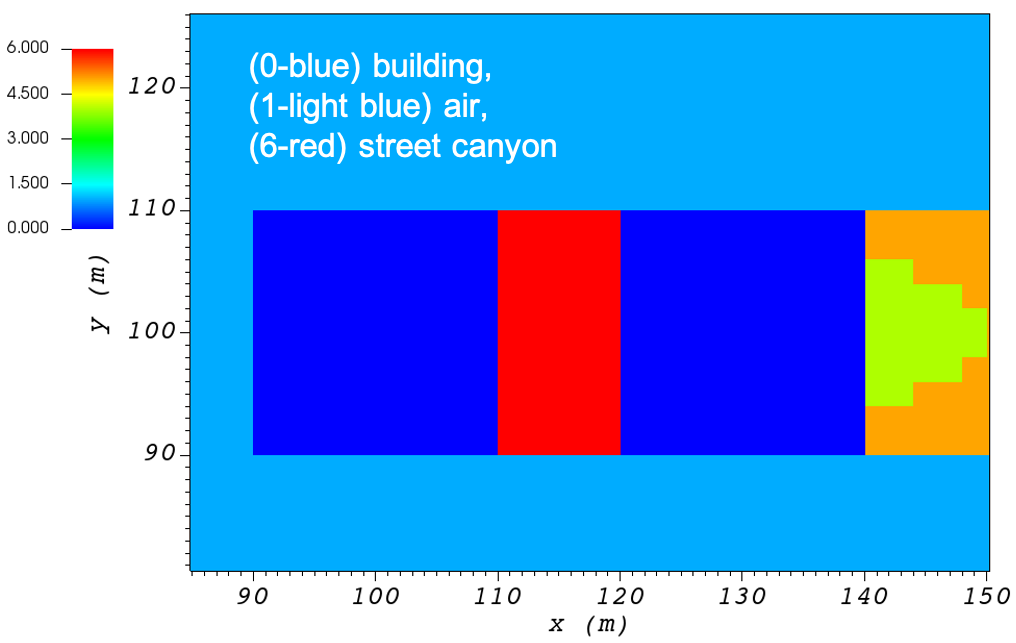
\includegraphics[width=10.3cm,keepaspectratio]{Images/street_z_5_1_init_icell.png}
    \caption{Cell type}
    \end{subfigure}
    \begin{subfigure}[t]{0.45\textwidth}
    \centering
    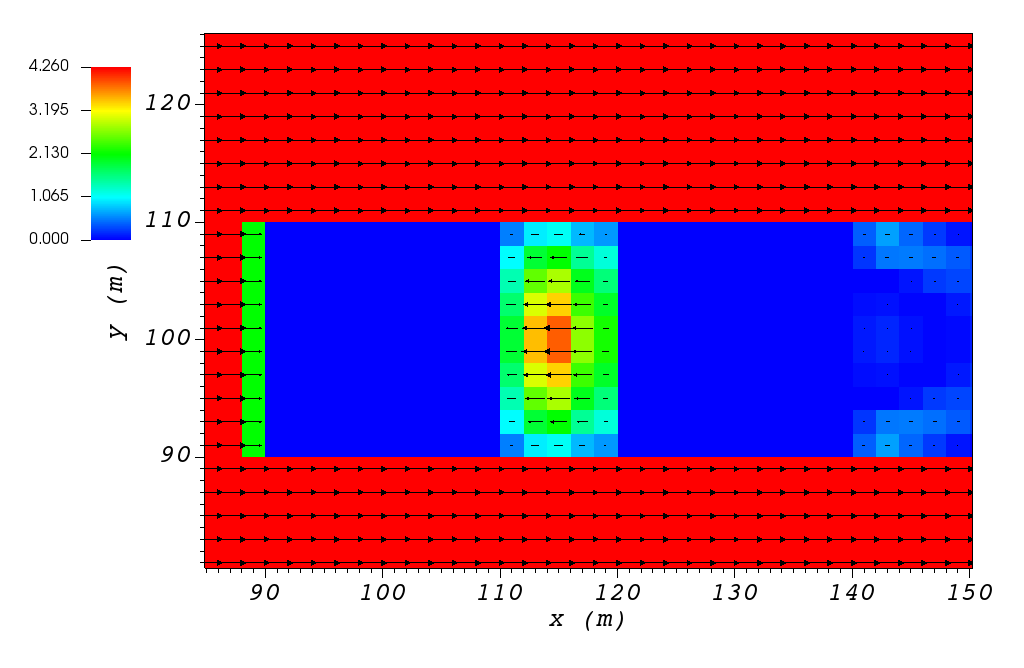
\includegraphics[width=11.0cm,keepaspectratio]{Images/street_z_5_1_init_vel.png}
    \caption{Initial velocity field}
    \end{subfigure}
    \begin{subfigure}[t]{0.45\textwidth}
    \centering
    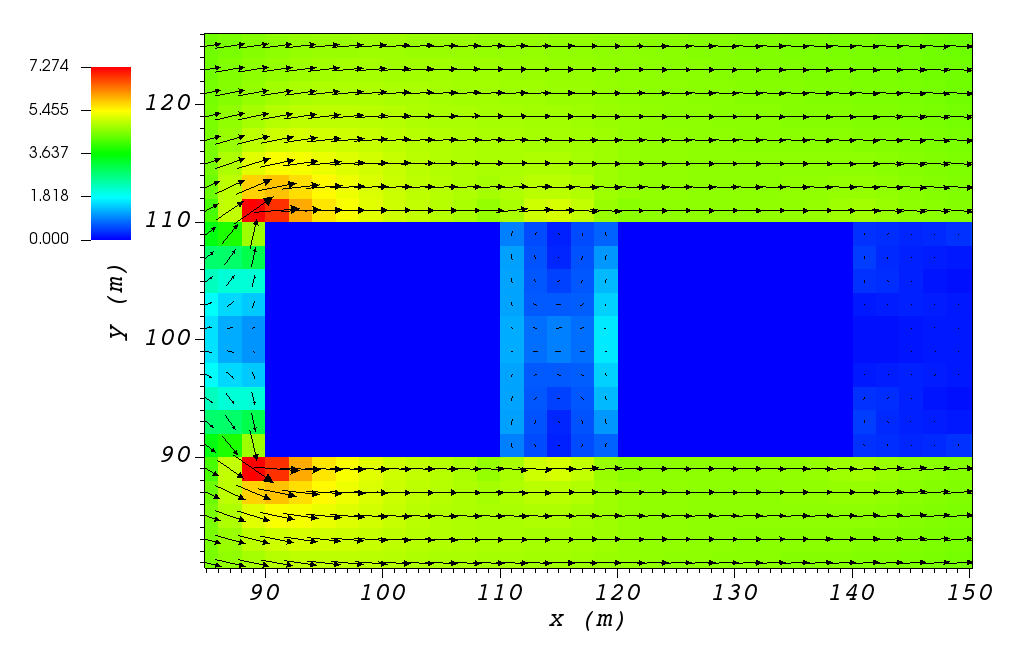
\includegraphics[width=11.0cm,keepaspectratio]{Images/street_z_5_1_final.png}
    \caption{Final velocity field}
    \end{subfigure}
\end{figure}


\begin{figure}[p]
    \centering
    \begin{subfigure}[t]{0.45\textwidth}
    \centering
    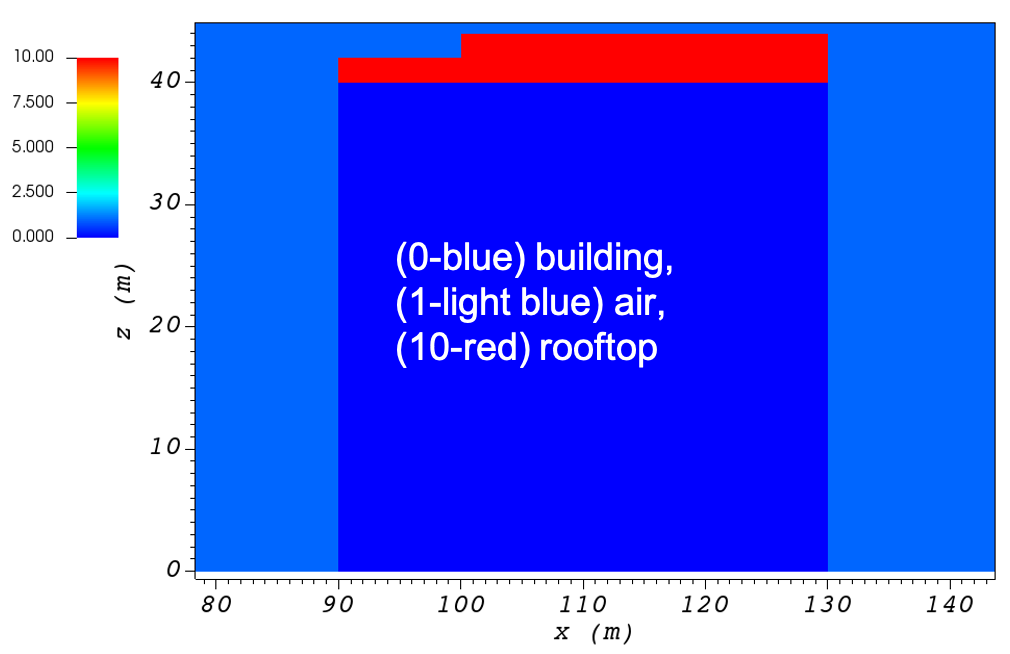
\includegraphics[width=10.3cm,keepaspectratio]{Images/rooftop_y_100_1_init_icell.png}
    \caption{Cell type}
    \end{subfigure}
    \begin{subfigure}[t]{0.45\textwidth}
    \centering
    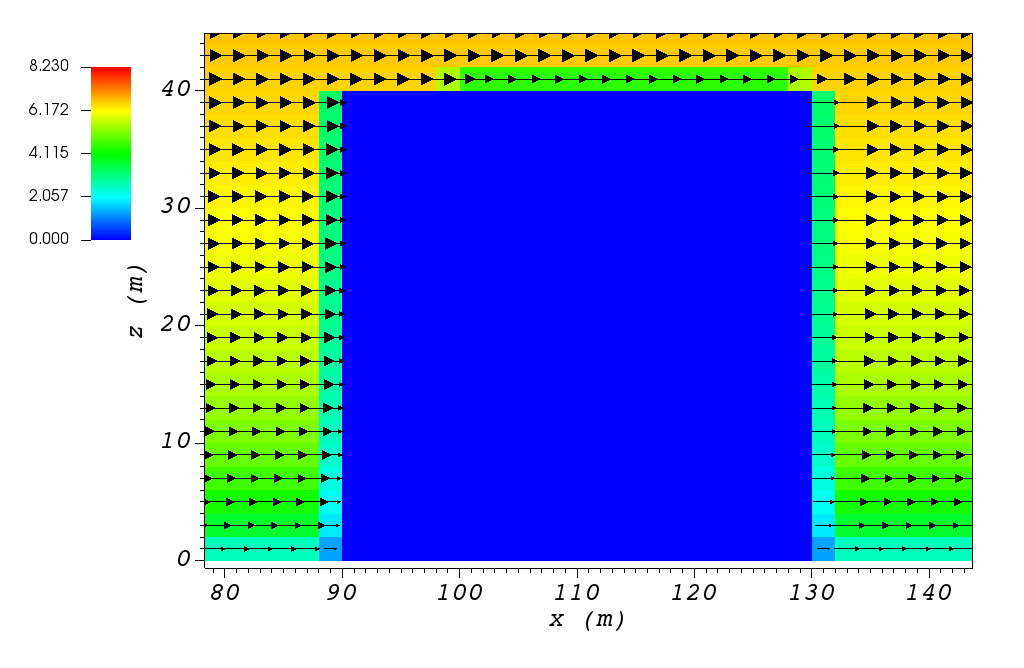
\includegraphics[width=11.0cm,keepaspectratio]{Images/rooftop_y_100_1_init_vel.png}
    \caption{Initial velocity field}
    \end{subfigure}
    \begin{subfigure}[t]{0.45\textwidth}
    \centering
    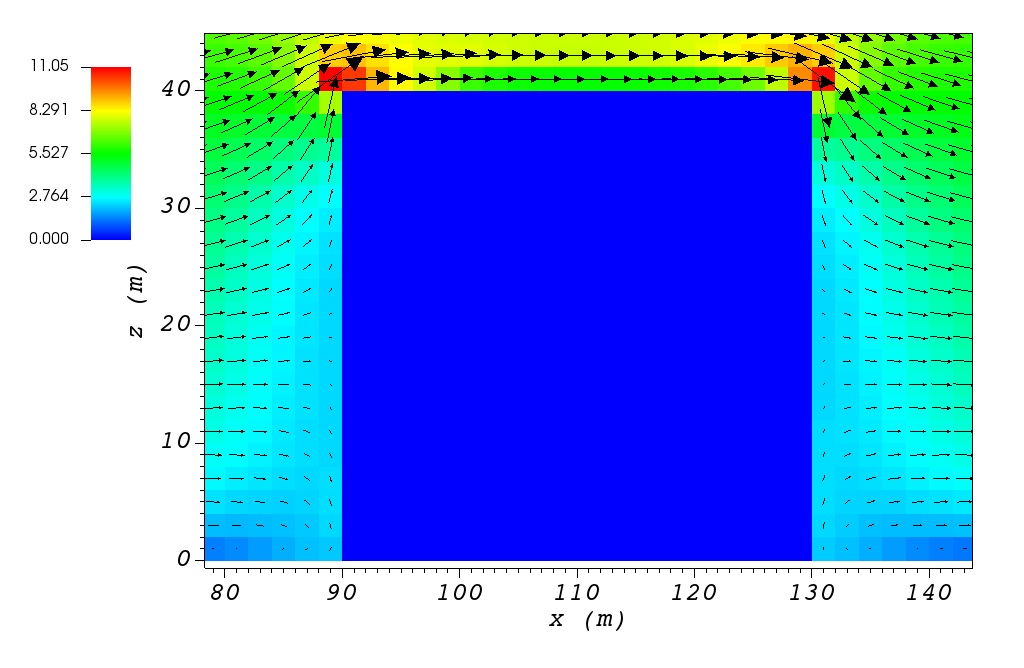
\includegraphics[width=11.0cm,keepaspectratio]{Images/rooftop_y_100_1_final.png}
    \caption{Final velocity field}
    \end{subfigure}
\end{figure}


\begin{figure}[p]
    \centering
    \begin{subfigure}[t]{0.45\textwidth}
    \centering
    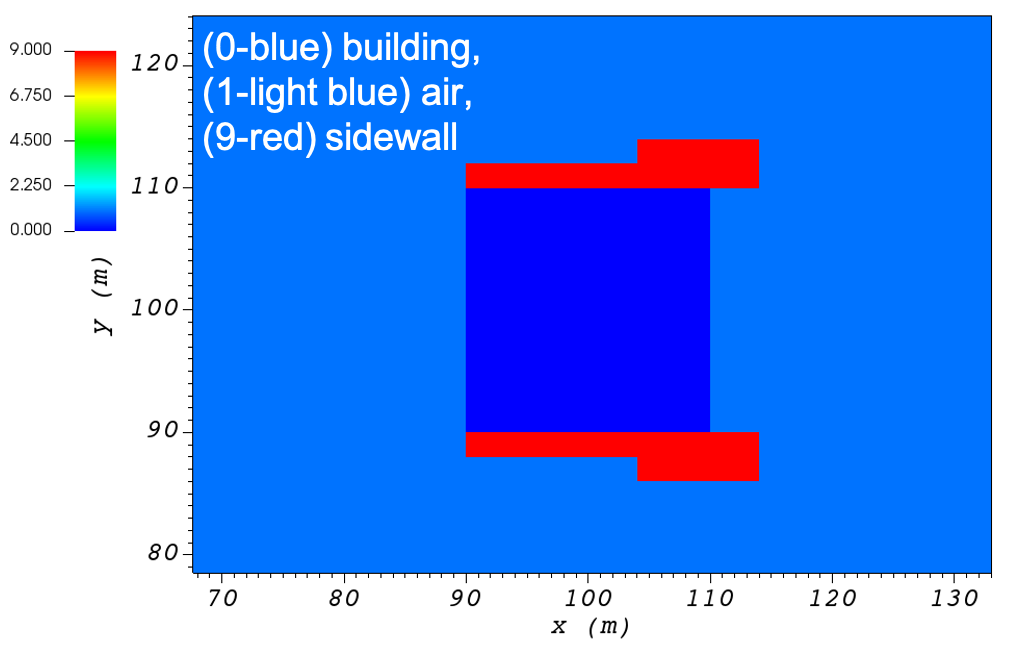
\includegraphics[width=10.3cm,keepaspectratio]{Images/sidewall_z_5_1_init_icell.png}
    \caption{Cell type}
    \end{subfigure}
    \begin{subfigure}[t]{0.45\textwidth}
    \centering
    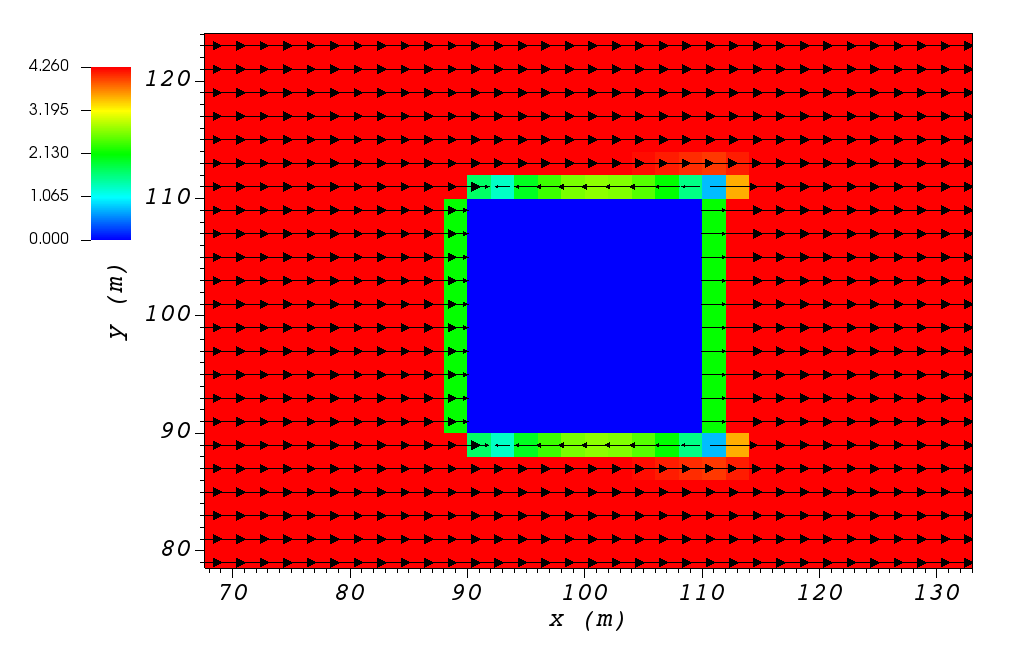
\includegraphics[width=11.0cm,keepaspectratio]{Images/sidewall_z_5_1_init_vel.png}
    \caption{Initial velocity field}
    \end{subfigure}
    \begin{subfigure}[t]{0.45\textwidth}
    \centering
    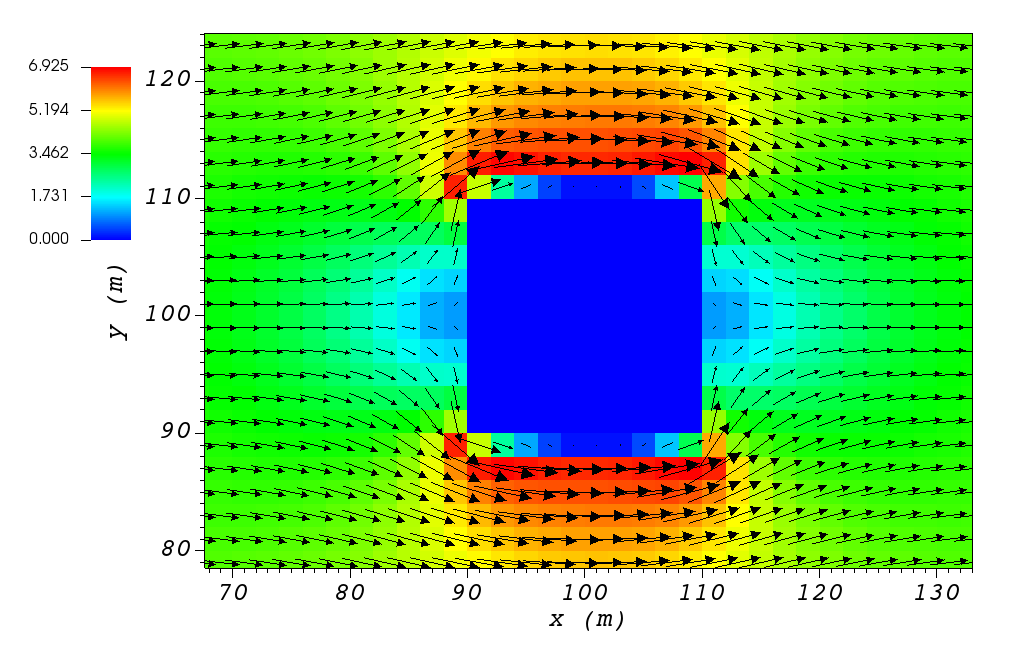
\includegraphics[width=11.0cm,keepaspectratio]{Images/sidewall_z_5_1_final.png}
    \caption{Final velocity field}
    \end{subfigure}
\end{figure}

\end{document}